\documentclass[CT4S-EN-RU]{subfiles}

\begin{document}

\section{\caseENGRUS{Finite limits in $\Set$}{ / }{Конечные пределы в $\Set$}}\label{sec:finite limits}

\begin{blockENG}
In this section we discuss what are called {\em limits} of variously-shaped diagrams of sets. We will make all this much more precise when we discuss limits in arbitrary categories in Section \ref{sec:lims and colims in a cat}.
\end{blockENG}

\begin{blockRUS}
В этом разделе мы обсудим то, что называется {\em пределами} различной формы для диаграмм множеств. Впоследствии мы проделаем это же значительно более точно при обсуждении пределов в произвольных категориях в Разделе \ref{sec:lims and colims in a cat}.
\end{blockRUS}

%%%% Subsection %%%%

\subsection{\caseENGRUS{Pullbacks}{ / }{Пулбеки и притягивающие квадраты}}

\begin{definitionENG}[Pullback]\label{def:pullback}\index{pullback!of sets}
Suppose given the diagram of sets and functions below.
\begin{align}\label{dia:fp sets}
\xymatrix{&Y\ar[d]^g\\
X\ar[r]_f&Z}
\end{align}
Its {\em fiber product}\index{fiber product} is the set 
$$X\times_ZY:=\{(x,w,y)\|f(x)=w=g(y)\}.$$ There are obvious projections $\pi_1\taking X\times_ZY\to X$ and $\pi_2\taking X\times_ZY\to Y$ (e.g. $\pi_2(x,w,y)=y$). Note that if $W=X\times_ZY$ then the diagram 
\begin{align}\label{dia:pullback sets}
\xymatrix{W\ullimit\ar[r]^-{\pi_2}\ar[d]_{\pi_1}&Y\ar[d]^g\\
X\ar[r]_f&Z}
\end{align}
commutes. Given the setup of Diagram \ref{dia:fp sets} we define the {\em pullback of $X$ and $Y$ over $Z$} to be any set $W$ for which we have an isomorphism $W\To{\iso}X\times_ZY$. The corner symbol $\lrcorner$ in Diagram \ref{dia:pullback sets} indicates that $W$ is the pullback.\index{a symbol!$\lrcorner$}
\end{definitionENG}

\begin{definitionRUS}[Притягивающий квадрат]\label{def:pullback}\index{притягивающий квадрат!множеств}\index{пулбек!множеств}\index{расслоенное произведение!множеств}
Предположим, дана следующая диаграмма множеств и функций:
\begin{align}\label{dia:fp sets}
\xymatrix{&Y\ar[d]^g\\
X\ar[r]_f&Z}
\end{align}
Ее {\em расслоенное произведение}\index{расслоенное произведение} — это множество 
$$X\times_ZY:=\{(x,w,y)\|f(x)=w=g(y)\}.$$ 
Имеются очевидные проекции $\pi_1\taking X\times_ZY\to X$ и $\pi_2\taking X\times_ZY\to Y$ (например, $\pi_2(x,w,y)=y$). Заметим, что если $W=X\times_ZY$, то диаграмма 
\begin{align}\label{dia:pullback sets}
\xymatrix{W\ullimit\ar[r]^-{\pi_2}\ar[d]_{\pi_1}&Y\ar[d]^g\\
X\ar[r]_f&Z}
\end{align}
коммутирует. В контексте Диаграммы \ref{dia:fp sets} мы определяем {\em пулбек $X$ и $Y$ над $Z$} как любое множество $W$, для которого имеется изоморфизм $W\To{\iso}X\times_ZY$. Символ-уголок $\lrcorner$ в Диаграмме \ref{dia:pullback sets} отражает то, что $W$ является пулбеком; такие диаграммы называются {\em притягивающими квадратами}.\index{символ!$\lrcorner$}
\end{definitionRUS}

\begin{exerciseENG}
Let $X,Y,Z$ be as drawn and $f\taking X\to Z$ and $g\taking Y\to Z$ the indicated functions. 
\begin{center}
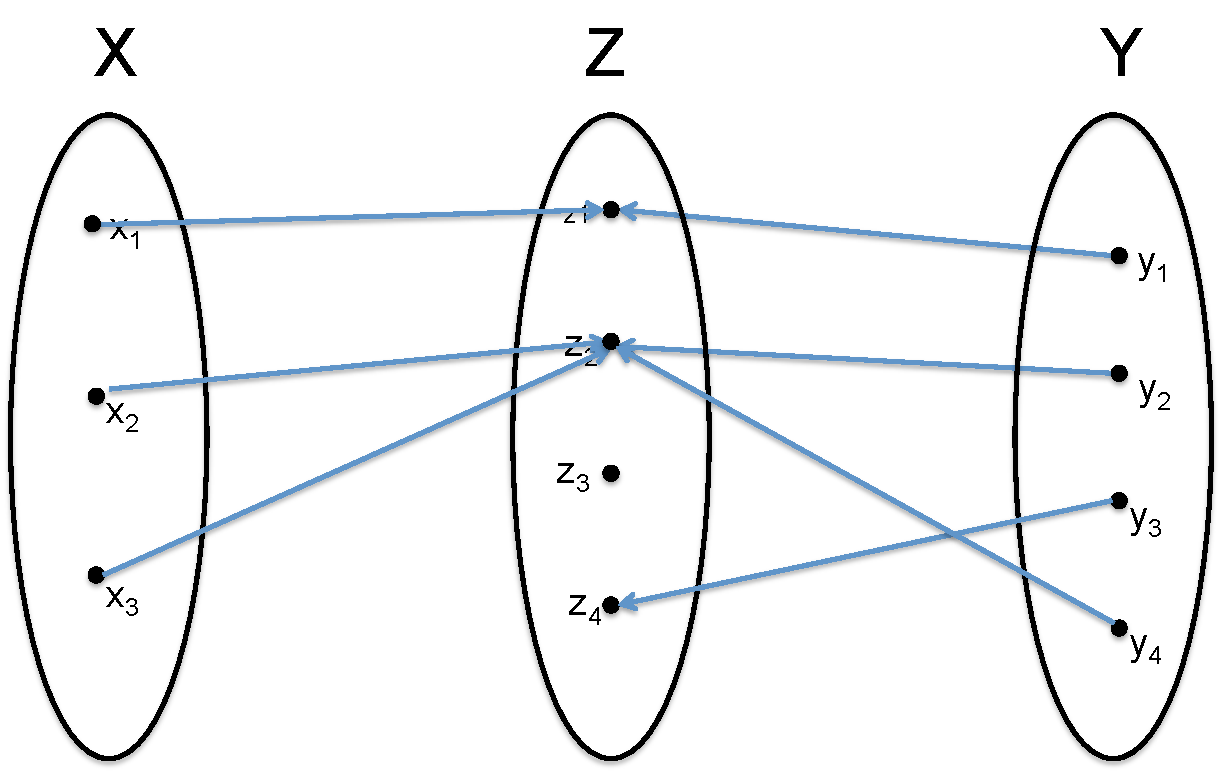
\includegraphics[height=2in]{setPullback}
\end{center}
What is the pullback of the diagram $X\Too{f}Z\Fromm{g}Y$?
\end{exerciseENG}

\begin{exerciseRUS}
Пусть $X,Y,Z$ такие, как на рисунке, а $f\taking X\to Z$ и $g\taking Y\to Z$ — изображенные функции. 
\begin{center}
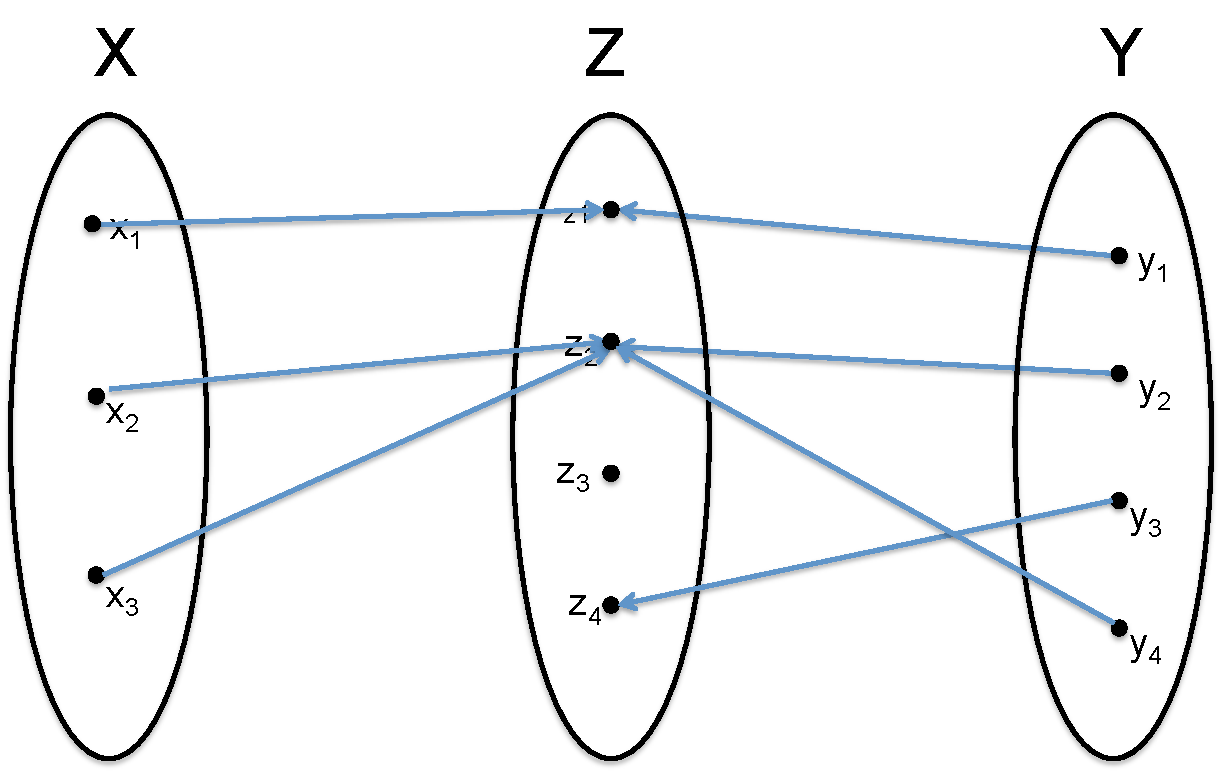
\includegraphics[height=2in]{setPullback}
\end{center}
Каким будет пулбек диаграммы $X\Too{f}Z\Fromm{g}Y$?
\end{exerciseRUS}

\begin{exerciseENG}~
\sexc Draw a set $X$ with five elements and a set $Y$ with three elements. Color each element of $X$ and each element of $Y$ either red, blue, or yellow,%
\footnote{You can use shadings rather than coloring, if coloring would be annoying.}
and do so in a “random-looking” way. Considering your coloring of $X$ as a function $X\to C$, where $C=\{\tn{red, blue, yellow}\}$, and similarly obtaining a function $Y\to C$, draw the fiber product $X\times_CY$. Make sure it is colored appropriately.
\item The universal property for products guarantees a function $X\times_CY\to X\times Y$, which I can tell you will be an injection. This means that the drawing you made of the fiber product can be imbedded into the $5\times 3$ grid; please draw the grid and indicate this subset.
\endsexc
\end{exerciseENG}

\begin{exerciseRUS}~
\sexc Нарисуйте множество $X$ из пяти элементов и множество $Y$ из трех элементов. Раскрасьте все элементы $X$ и $Y$ либо в красный, либо в синий, либо в желтый цвет,%
\footnote{Можете их заштриховать, а не раскрашивать, если раскрашивать вам неудобно.}
причем сделайте это «случайным» образом. Считая вашу раскраску $X$ функцией $X\to C$, где $C=\{\tn{красный, синий, желтый}\}$, и аналогичным образом получив функцию $Y\to C$, нарисуйте расслоенное произведение $X\times_CY$. Раскрасив его подходящим образом, убедитесь, что цвета пар совпадают.
\item Универсальное свойство произведений обеспечивает нам функцию $X\times_CY\to X\times Y$, которая, можете мне поверить, будет инъекцией. Это означает, что рисунок расслоенного произведения, который вы сделали, может быть вставлен в сетку $5\times 3$; изобразите, пожалуйста, такую сетку и отметьте на ней подмножество.
\endsexc
\end{exerciseRUS}

\begin{remarkENG}
Some may prefer to denote this fiber product by $f\times_Zg$ rather than $X\times_ZY$. The former is  mathematically better notation, but human-readability is often enhanced by the latter, which is also more common in the literature. We use whichever is more convenient.
\end{remarkENG}

\begin{remarkRUS}
Некоторые предпочитают обозначать расслоенное произведение $f\times_Zg$, а не $X\times_ZY$. Первое обозначение математически корректнее, но читабельность для человека часто лучше у второго, которое, кроме того, чаще встречается в литературе. Мы будем использовать такое обозначение, которое окажется более удобным.
\end{remarkRUS}

\begin{exerciseENG}~
\sexc Suppose that $Y=\emptyset$; what can you say about $X\times_ZY$? 
\item Suppose now that $Y$ is any set but that $Z$ has exactly one element; what can you say about $X\times_ZY$?
\endsexc
\end{exerciseENG}

\begin{exerciseRUS}~
\sexc Предположим, что $Y=\varnothing$; что вы можете сказать о $X\times_ZY$? 
\item Предположим теперь, что $Y$ — любое множество, а $Z$ имеет в точности один элемент; что вы можете сказать о $X\times_ZY$?
\endsexc
\end{exerciseRUS}

\begin{exerciseENG}
Let $S=\RR^3, T=\RR$, and think of them as (Aristotelian) space and time, with the origin in $S\times T$ given by the center of mass of MIT at the time of its founding. Let $Y=S\times T$ and let $g_1\taking Y\to S$ be one projection and $g_2\taking Y\to T$ the other projection. Let $X=\singleton$ be a set with one element and let $f_1\taking X\to S$ and $f_2\taking X\to T$ be given by the origin in both cases. 
\sexc What are the fiber products $W_1$ and $W_2$:
$$
\xymatrix{W_1\ar[r]\ar[d]\ullimit&Y\ar[d]^{g_1}\\X\ar[r]_{f_1}&S}\hspace{1in}
\xymatrix{W_2\ar[r]\ar[d]\ullimit&Y\ar[d]^{g_2}\\X\ar[r]_{f_2}&T}
$$
\item Interpret these sets in terms of the center of mass of MIT at the time of its founding.
\endsexc
\end{exerciseENG}

\begin{exerciseRUS}
Пусть $S=\RR^3, T=\RR$, будем думать о них, как об (Аристотелевых) пространстве и времени, с началом отсчета в $S\times T$, заданным центром масс [университета] MIT в момент его основания. Пусть $Y=S\times T$ и $g_1\taking Y\to S$ — одна из проекций, а $g_2\taking Y\to T$ — другая. Пусть $X=\singleton$ — множество из одного элемента, а $f_1\taking X\to S$ и $f_2\taking X\to T$ заданы как начала отсчета в обоих случаях. 
\sexc Какими будут расслоенные произведения $W_1$ и $W_2$:
$$
\xymatrix{W_1\ar[r]\ar[d]\ullimit&Y\ar[d]^{g_1}\\X\ar[r]_{f_1}&S}\hspace{1in}
\xymatrix{W_2\ar[r]\ar[d]\ullimit&Y\ar[d]^{g_2}\\X\ar[r]_{f_2}&T}
$$
\item Интерпретируйте эти множества в терминах центра масс MIT в момент его основания.
\endsexc
\end{exerciseRUS}

%% Subsubsection %%

\subsubsection{\caseENGRUS{Using pullbacks to define new ideas from old}{ / }{Использование пуллбеков для определения новый идей на основе старых}}

\begin{blockENG}
In this section we will see that the fiber product of a diagram can serve to define a new concept. For example, in (\ref{dia:bad battery}) we define what it means for a cellphone to have a bad battery, in terms of the length of time for which it remains charged. By being explicit, we reduce the chance of misunderstandings between different groups of people. This can be useful in situations like audits and those in which one is trying to reuse or understand data gathered by others.
\end{blockENG}

\begin{blockRUS}
В этом разделе мы увидим, что расслоенное произведение диаграммы может послужить нам для того, чтобы определить новое понятие. Например, в (\ref{dia:bad battery}) мы определяем, что такое мобильный телефон с плохим аккумулятором, в терминах продолжительности времени, которое он остается заряженным. Выражая вещи более явно, мы уменьшаем шанс возникновения недопониманий между различными группами людей. Это может быть полезно в ситуациях вроде аудита, либо когда некто пытается использовать и понять данные, собранные другими.
\end{blockRUS}

\begin{exampleENG}
Consider the following two ologs. The one on the right is the pullback of the one on the left. 
\begin{align}\label{dia:wealthy and loyal}
\fbox{\xymatrixnocompile{&\obox{C}{.7in}{\rr a loyal customer}\LA{d}{is}\\\obox{B}{.7in}{\rr a wealthy customer}\LA{r}{is}&\smbox{D}{a customer}}}\hsp&\fbox{\xymatrix{\obox{A=B\times_DC}{.9in}{\rr a customer that is wealthy and loyal}\LAL{d}{is}\LA{r}{is}&\obox{C}{.7in}{\rr a loyal customer}\LA{d}{is}\\\obox{B}{.7in}{\rr a wealthy customer}\LA{r}{is}&\smbox{D}{a customer}}}
\end{align}
Check from Definition \ref{def:pullback} that the label, “a customer that is wealthy and loyal”, is fair and straightforward as a label for the fiber product $A=B\times_DC$, given the labels on $B,C$, and $D$.
\end{exampleENG}

\begin{exampleRUS}
Рассмотрим следующие два олога. Тот, что справа, является притягивающим квадратом того, что слева. 
\begin{align}\label{dia:wealthy and loyal}
\fbox{\xymatrixnocompile{&\obox{C}{.7in}{\rr лояльный потребитель}\LA{d}{это}\\\obox{B}{.7in}{\rr богатый потребитель}\LA{r}{это}&\smbox{D}{потребитель}}}\hsp&\fbox{\xymatrix{\obox{A=B\times_DC}{.9in}{\rr богатый и лояльный потребитель}\LAL{d}{это}\LA{r}{это}&\obox{C}{.7in}{\rr лояльный потребитель}\LA{d}{это}\\\obox{B}{.7in}{\rr богатый потребитель}\LA{r}{это}&\smbox{D}{потребитель}}}
\end{align}
Проверьте по определению \ref{def:pullback}, что метка «богатый и лояльный потребитель» — это корректная и достаточно прямолинейная метка для расслоенного произведения $A=B\times_DC$, если на $B,C$ и $D$ поставить соответствующие метки.%
\endnote{
С точки зрения теории множеств, мы только что построили пересечение двух подмножеств одного множества. В общем случае, такие пересечения моделируются в теории категорий именно притягивающими квадратами.
}
\end{exampleRUS}

\begin{remarkENG}\label{rem:defining using pullbacks}
Note that in Diagram (\ref{dia:wealthy and loyal}) the top-left box could have been (non-canonically named) \fakebox{a good customer}. If it was taken to be the fiber product, then the author would be effectively {\em defining} a good customer to be one that is wealthy and loyal. 
\end{remarkENG}

\begin{remarkRUS}\label{rem:defining using pullbacks}
Заметим, что в Диаграмме (\ref{dia:wealthy and loyal}) верхний левый прямоугольник может быть (неканонически) назван \fakebox{хороший потребитель}. Если указать именно его в качестве пулбека, то автор [олога] будет фактически {\em определять} хорошего потребителя как того, кто одновременно богат и покорен. 
\end{remarkRUS}

\begin{exerciseENG}
For each of the following, an author has proposed that the diagram on the right is a pullback. Do you think their labels are appropriate or misleading; that is, is the label on the upper-left box reasonable given the rest of the olog, or is it suspect in some way?
\sexc\begin{align*}\footnotesize\fbox{\xymatrix{&&\smbox{C}{blue}\LA{d}{is}\\\smbox{B}{a person}\LA{rr}{\parbox{.7in}{\rr has as favorite color}}&&\smbox{D}{a color}}}\hsp&\footnotesize\fbox{\xymatrixnocompile{\obox{A=B\times_DC}{1.1in}{\rr a person whose favorite color is blue}\LAL{d}{is}\LA{rr}{\parbox{.7in}{\rr has as favorite color}}&&\smbox{C}{blue}\LA{d}{is}\\\smbox{B}{a person}\LA{rr}{\parbox{.7in}{\rr has as favorite color}}&&\smbox{D}{a color}}}
\end{align*}
\item\begin{align*}\footnotesize\fbox{\xymatrixnocompile{&&\smbox{C}{a woman}\LA{d}{is}\\\smbox{B}{a dog}\LA{rr}{\parbox{.7in}{\rr has as owner}}&&\smbox{D}{a person}}}\hsp&\footnotesize\fbox{\xymatrixnocompile{\obox{A=B\times_DC}{1in}{\rr a dog whose owner is a woman}\LAL{d}{is}\LA{rr}{\parbox{.7in}{\rr has as owner}}&&\smbox{C}{a woman}\LA{d}{is}\\\smbox{B}{a dog}\LA{rr}{\parbox{.7in}{\rr has as owner}}&&\smbox{D}{a person}}}
\end{align*}
\item\begin{align*}\footnotesize\fbox{\xymatrixnocompile{&\obox{C}{.5in}{\rr a piece of furniture}\LA{d}{has}\\\obox{B}{.6in}{\rr a space in our house}\LA{r}{has}&\smbox{D}{a width}}}\hsp&\footnotesize\fbox{\xymatrixnocompile{\obox{A=B\times_DC}{.5in}{\rr a good fit}\LAL{d}{$s$}\LA{r}{$f$}&\obox{C}{.5in}{\rr a piece of furniture}\LA{d}{has}\\\obox{B}{.6in}{\rr a space in our house}\LA{r}{has}&\smbox{D}{a width}}}
\end{align*}
\endsexc
\end{exerciseENG}

\begin{exerciseRUS}
Для каждого из нижеследующих [ологов] автор заявляет, что диаграмма справа является притягивающим квадратом. Считаете ли вы метки подходящими или сбивающими с толку; другими словами, будет ли метка на верхнем левом прямоугольнике обоснованой остальной частью олога или же она некоторым образом вызывает подозрение?
\sexc\begin{align*}\footnotesize\fbox{\xymatrix{&&\smbox{C}{синий}\LA{d}{это}\\\smbox{B}{человек}\LA{rr}{\parbox{.7in}{\rr любимый цвет}}&&\smbox{D}{цвет}}}\hsp&\footnotesize\fbox{\xymatrixnocompile{\obox{A=B\times_DC}{1.1in}{\rr человек, который любит синий цвет}\LAL{d}{это}\LA{rr}{\parbox{.7in}{\rr любимый цвет}}&&\smbox{C}{синий}\LA{d}{это}\\\smbox{B}{человек}\LA{rr}{\parbox{.7in}{\rr любимый цвет}}&&\smbox{D}{цвет}}}
\end{align*}
\item\begin{align*}\footnotesize\fbox{\xymatrixnocompile{&&\smbox{C}{женщина}\LA{d}{это}\\\smbox{B}{собака}\LA{rr}{\parbox{.7in}{\rr владелец}}&&\smbox{D}{человек}}}\hsp&\footnotesize\fbox{\xymatrixnocompile{\obox{A=B\times_DC}{1in}{\rr собака, у которой владелец — женщина}\LAL{d}{это}\LA{rr}{\parbox{.7in}{\rr владелец}}&&\smbox{C}{женщина}\LA{d}{это}\\\smbox{B}{собака}\LA{rr}{\parbox{.7in}{\rr владелец}}&&\smbox{D}{человек}}}
\end{align*}
\item\begin{align*}\footnotesize\fbox{\xymatrixnocompile{&\obox{C}{.5in}{\rr предмет мебели}\LA{d}{имеет}\\\obox{B}{.6in}{\rr свободное место в доме}\LA{r}{имеет}&\smbox{D}{ширина}}}\hsp&\footnotesize\fbox{\xymatrixnocompile{\obox{A=B\times_DC}{.5in}{\rr подходит}\LAL{d}{$s$}\LA{r}{$f$}&\obox{C}{.5in}{\rr предмет мебели}\LA{d}{имеет}\\\obox{B}{.6in}{\rr свободное место в доме}\LA{r}{имеет}&\smbox{D}{ширина}}}
\end{align*}
\endsexc
\end{exerciseRUS}

\begin{exerciseENG}~
\sexc Consider your olog from Exercise \ref{exc:family olog}. Are any of the commutative squares there actually pullback squares? 
\item Now use ologs with products and pullbacks to define what a brother is and what a sister is (again in a human biological nuclear family), in terms of types such as \fakebox{an offspring of mating pair $(a,b)$}, \fakebox{a person}, \fakebox{a male person}, \fakebox{a female person}, and so on.
\endsexc
\end{exerciseENG}

\begin{exerciseRUS}~
\sexc Рассмотрите свой олог из Упражнения \ref{exc:family olog}. Будут ли какие-либо из коммутативных квадратов в нем притягивающими? 
\item Теперь используйте ологи с произведениями и пулбеками, чтобы определить, что такое брат, и что такое сестра (опять же, в человеческой биологической нуклеарной семье), в терминах типов, таких как \fakebox{потомок супружеской пары $(a,b)$}, \fakebox{человек}, \fakebox{мужчина}, \fakebox{женщина}, и им подобных.
\endsexc
\end{exerciseRUS}

\begin{definitionENG}[Preimage]\label{def:preimage}
Let $f\taking X\to Y$ be a function and $y\in Y$ an element. The {\em preimage of y under $f$}\index{preimage}, denoted $f^\m1(y)$,\index{a symbol!$f^\m1$} is  the subset $f^\m1(y):=\{x\in X\|f(x)=y\}$. If $Y'\ss Y$ is any subset, the {\em preimage of $Y'$ under $f$}, denoted $f^\m1(Y')$, is the subset $f^\m1(Y')=\{x\in X\|f(x)\in Y'\}$.
\end{definitionENG}

\begin{definitionRUS}[Прообраз]\label{def:preimage}
Пусть $f\taking X\to Y$ — функция и $y\in Y$ — элемент. {\em Прообраз $y$ относительно $f$}\index{прообраз}, обозначаемый $f^\m1(y)$,\index{символ!$f^\m1$} — это подмножество $f^\m1(y):=\{x\in X\|f(x)=y\}$. Если $Y'\ss Y$ — произвольное подмножество, то {\em прообраз $Y'$ относительно $f$}, обозначаемый $f^\m1(Y')$, — это подмножество $f^\m1(Y')=\{x\in X\|f(x)\in Y'\}$.
\end{definitionRUS}

\begin{exerciseENG}
Let $f\taking X\to Y$ be a function and $y\in Y$ an element. Draw a pullback diagram in which the fiber product is isomorphic to the preimage $f^\m1(y)$.
\end{exerciseENG}

\begin{exerciseRUS}
Пусть $f\taking X\to Y$ — функция и $y\in Y$ — элемент. Нарисуйте притягивающий квадрат, в котором расслоенное произведение изоморфно прообразу $f^\m1(y)$. 
\end{exerciseRUS}

\begin{lemmaENG}[Universal property for pullback]\label{lemma:up for fp}
Suppose given the diagram of sets and functions as below.
\begin{align*}
\xymatrix{&Y\ar[d]^u\\
X\ar[r]_t&Z}
\end{align*}
For any set $A$ and commutative solid arrow diagram as below (i.e. functions $f\taking A\to X$ and $g\taking A\to Y$ such that $t\circ f=u\circ g$), 
\begin{align}\label{dia:universal property of fp}
\xymatrix{
&X\times_ZY\ar@/_1pc/[lddd]_{\pi_1}\ar@/^1pc/[rddd]^{\pi_2}\\\\
&A\ar@{-->}[uu]^{\exists!}\ar[dl]_{\forall f}\ar[dr]^{\forall g}&\\
X\ar[rd]_t&&Y\ar[ld]^u\\
&Z&}
\end{align}
there exists a unique arrow $\pb{f}{g}{Z}\taking A\to X\times_ZY$ making everything commute, i.e. 
$$f=\pi_1\circ \pb{f}{g}{Z}\hsp\text{and}\hsp g=\pi_2\circ\pb{f}{g}{Z}.$$
\end{lemmaENG}

\begin{lemmaRUS}[Универсальное свойство притягивающего квадрата]\label{lemma:up for fp}
Предположим, дана следующая диаграмма множеств и функций.
\begin{align*}
\xymatrix{&Y\ar[d]^u\\
X\ar[r]_t&Z}
\end{align*}
Для любого множества $A$ и коммутативной диаграммы из непрерывных стрелок, данной ниже (т.е. функций $f\taking A\to X$ и $g\taking A\to Y$ таких, что $t\circ f=u\circ g$), 
\begin{align}\label{dia:universal property of fp}
\xymatrix{
&X\times_ZY\ar@/_1pc/[lddd]_{\pi_1}\ar@/^1pc/[rddd]^{\pi_2}\\\\
&A\ar@{-->}[uu]^{\exists!}\ar[dl]_{\forall f}\ar[dr]^{\forall g}&\\
X\ar[rd]_t&&Y\ar[ld]^u\\
&Z&}
\end{align}
существует единственная стрелка $\pb{f}{g}{Z}\taking A\to X\times_ZY$, делающая коммутативным все остальное, т.е.
$$f=\pi_1\circ \pb{f}{g}{Z}\hsp\text{и}\hsp g=\pi_2\circ\pb{f}{g}{Z}.$$
\end{lemmaRUS}

\begin{exerciseENG}
Create an olog whose underlying shape is a commutative square. Now add the fiber product so that the shape is the same as that of Diagram (\ref{dia:universal property of fp}). Assign English labels to the projections $\pi_1,\pi_2$ and to the dotted map $A\To{\pb{f}{g}{Z}}X\times_ZY$, such that these labels are as canonical as possible.
\end{exerciseENG}

\begin{exerciseRUS}
Постройте олог с произвольной коммутативной диаграммой. Теперь добавьте расслоенное произведение так, чтобы форма диаграммы стала подобной Диаграмме (\ref{dia:universal property of fp}). Дайте метки на естественном языке проекциям $\pi_1,\pi_2$ и пунктирному отображению $A\To{\pb{f}{g}{Z}}X\times_ZY$ таким образом, чтобы эти метки были по возможности каноничны.
\end{exerciseRUS}

%% Subsubsection %%

\subsubsection{\caseENGRUS{Pasting diagrams for pullback}{ / }{Склеивание диаграмм для пуллбеков}}

\begin{blockENG}
Consider the diagram drawn below, which includes a left-hand square, a right-hand square, and a big rectangle.
$$
\xymatrix{
A'\ar[r]^{f'}\ar[d]_i\ullimit&B'\ar[r]^{g'}\ar[d]_j\ullimit&C'\ar[d]^k\\
A\ar[r]_f&B\ar[r]_g&C}
$$
The right-hand square has a corner symbol indicating that $B'\iso B\times_CC'$ is a pullback. But the corner symbol on the left is ambiguous; it might be indicating that the left-hand square is a pullback, or it might be indicating that the big rectangle is a pullback. It turns out that if $B'\iso B\times_CC'$ then it is not ambiguous because the left-hand square is a pullback if and only if the big rectangle is.
\end{blockENG}

\begin{blockRUS}
Рассмотрим диаграмму, изображенную ниже, которая включает коммутативные квадраты слева, справа, а также [обрамляющий их] большой прямоугольник.
$$
\xymatrix{
A'\ar[r]^{f'}\ar[d]_i\ullimit&B'\ar[r]^{g'}\ar[d]_j\ullimit&C'\ar[d]^k\\
A\ar[r]_f&B\ar[r]_g&C}
$$
Квадрат справа имеет символ-уголок, означающий, что $B'\iso B\times_CC'$ — пулбек. Но символ-уголок слева неоднозначен; он мог бы относиться и к левому квадрату, и к большому прямоугольнику. Однако оказывается, что если $B'\iso B\times_CC'$, то разночтений нет, потому что левый квадрат является притягивающим тогда и только тогда, когда таковым является большой прямоугольник.
\end{blockRUS}

\begin{propositionENG}\label{prop:pasting}
Consider the diagram drawn below
$$
\xymatrix{
&B'\ar[r]^{g'}\ar[d]_j\ullimit&C'\ar[d]^k\\
A\ar[r]_f&B\ar[r]_g&C}
$$
where $B'\iso B\times_CC'$ is a pullback. Then there is an isomorphism $A\times_BB'\iso A\times_CC'$. Said another way, $$A\times_B(B\times_CC')\iso A\times_CC'.$$
\end{propositionENG}

\begin{propositionRUS}\label{prop:pasting}
Рассмотрим диаграмму, изображенную ниже
$$
\xymatrix{
&B'\ar[r]^{g'}\ar[d]_j\ullimit&C'\ar[d]^k\\
A\ar[r]_f&B\ar[r]_g&C}
$$
где $B'\iso B\times_CC'$ — пулбек. Тогда имеется изоморфизм $A\times_BB'\iso A\times_CC'$. Другими словами, $$A\times_B(B\times_CC')\iso A\times_CC'.$$
\end{propositionRUS}

\begin{proofENG}
We first provide a map $\phi\taking A\times_B(B\times_CC')\to A\times_CC'$. An element of $A\times_B(B\times_CC')$ is of the form $(a,b,(b,c,c'))$ such that $f(a)=b, g(b)=c$ and $k(c')=c$. But this implies that $g\circ f(a)=c=k(c')$ so we put $\phi(a,b,(b,c,c')):=(a,c,c')\in A\times_CC'$. Now we provide a proposed inverse, $\psi\taking A\times_CC'\to A\times_B(B\times_CC')$. Given $(a,c,c')$ with $g\circ f(a)=c=k(c')$, let $b=f(a)$ and note that $(b,c,c')$ is an element of $B\times_CC'$. So we can define $\psi(a,c,c')=(a,b,(b,c,c'))$. It is easy to see that $\phi$ and $\psi$ are inverse.
\end{proofENG}

\begin{proofRUS}
Сначала получим отображение $\phi\taking A\times_B(B\times_CC')\to A\times_CC'$. Элементы из $A\times_B(B\times_CC')$ имеют вид $(a,b,(b,c,c'))$ таких, что $f(a)=b, g(b)=c$ и $k(c')=c$. Но из этого следует, что $g\circ f(a)=c=k(c')$, так что мы можем положить $\phi(a,b,(b,c,c')):=(a,c,c')\in A\times_CC'$. Теперь получим необходимое обратное отображение $\psi\taking A\times_CC'\to A\times_B(B\times_CC')$. Для данного $(a,c,c')$ с $g\circ f(a)=c=k(c')$, пусть $b=f(a)$; заметим, что $(b,c,c')$ — элемент $B\times_CC'$. Поэтому мы можем определить $\psi(a,c,c')=(a,b,(b,c,c'))$. Легко видеть, что $\phi$ и $\psi$ будут взаимно обратными.
\end{proofRUS}

\begin{blockENG}
Proposition \ref{prop:pasting} can be useful in authoring ologs. For example, the type \fakebox{a cellphone that has a bad battery} is vague, but we can lay out precisely what it means using pullbacks:
\small
\begin{align}\label{dia:bad battery}
\fbox{\xymatrixnocompile{\obox{A\iso B\times_DC}{1in}{a cellphone that has a bad battery}\ar[r]\ar[d]&\smbox{C\iso D\times_FE}{a bad battery}\ar[r]\ar[d]&\obox{E\iso F\times_HG}{.5in}{less than 1 hour}\ar[r]\ar[d]&\obox{G}{.5in}{between 0 and 1}\ar[d]\\\smbox{B}{a cellphone}\LA{r}{has}&\smbox{D}{a battery}\LA{r}{\parbox{.4in}{\rr remains charged for}}&\obox{F}{.6in}{a duration of time}\LA{r}{\hspace{.07in}\parbox{.4in}{\rr in hours yields}}&\obox{H}{.6in}{a range of numbers}}}
\end{align}\normalsize
\end{blockENG}

\begin{blockRUS}
Утверждение \ref{prop:pasting} может оказаться полезным при создании ологов. Например, тип \fakebox{мобильный телефон с плохим аккумулятором} определен туманно, но мы можем точно сформулировать, что оно означает, используя пулбеки:
\small
\begin{align}\label{dia:bad battery}
\fbox{\xymatrixnocompile{\obox{A\iso B\times_DC}{1in}{мобильный телефон с плохим аккумулятором}\ar[r]\ar[d]&\smbox{C\iso D\times_FE}{плохой аккумулятор}\ar[r]\ar[d]&\obox{E\iso F\times_HG}{.5in}{менее 1 часа}\ar[r]\ar[d]&\obox{G}{.5in}{между 0 и 1}\ar[d]\\\smbox{B}{мобильный телефон}\LA{r}{имеет}&\smbox{D}{аккумулятор}\LA{r}{\parbox{.4in}{\rr остается заряженным}}&\obox{F}{.6in}{промежуток времени}\LA{r}{\hspace{.07in}\parbox{.4in}{\rr в часах}}&\obox{H}{.6in}{числовой промежуток}}}
\end{align}\normalsize
\end{blockRUS}

\begin{blockENG}
The category-theoretic fact described above says that since $A\iso B\times_DC$ and $C\iso D\times_FE$, it follows that $A\iso B\times_FE$.  That is, we can deduce the definition “a cellphone that has a bad battery is defined as a cellphone that has a battery which remains charged for less than one hour.”  
\end{blockENG}

\begin{blockRUS}
Теоретико-категорный факт, описанный выше, говорит, что из $A\iso B\times_DC$ и $C\iso D\times_FE$ следует $A\iso B\times_FE$. Это значит, мы можем вывести такое определение «мобильный телефон с плохим аккумулятором определяется как мобильный телефон, имеющий аккумулятор, который остается заряженным менее одного часа.»
\end{blockRUS}

\begin{exerciseENG}~
\sexc Create an olog that defines two people to be “of approximately the same height” if and only if their height difference is less than half an inch, using a pullback. Your olog can include the box \fakebox{a real number $x$ such that $-.5<x<.5$}. 
\item In the same olog, make a box for those people whose height is approximately the same as a person named “The Virgin Mary”. You may need to use images, as in Section \ref{sec:images}.
\endsexc
\end{exerciseENG}

\begin{exerciseRUS}~
\sexc Придумать олог, который при помощи пулбека определяет, что два человека «имеют приблизительно однаковый рост», если и только если разность их роста меньше половины дюйма. Ваш олог может включать прямоугольник \fakebox{действительное число $x$ такое, что $-.5<x<.5$}. 
\item В тот же олог добавьте прямоугольник для людей, чей рост приблизительно совпадает с ростом человека по имени «Дева Мария». Вам могут потребоваться образы функций, см. Раздел \ref{sec:images}.
\endsexc
\end{exerciseRUS}

\begin{exerciseENG}\label{exc:pointwise map of fp}
Consider the diagram on the left below, where both squares commute. 
$$
\xymatrix@=15pt{
&&&Y'\ar[dd]\\
&&Y\ar[ru]\ar[dd]\\
&X'\ar'[r][rr]&&Z'\\
X\ar[rr]\ar[ru]&&Z\ar[ru]
}
\hspace{1in}
\xymatrix@=15pt{
&W'\ar[rr]\ar'[d][dd]\ullimit&&Y'\ar[dd]\\
W\ar[rr]\ar[dd]\ullimit&&Y\ar[ru]\ar[dd]\\
&X'\ar'[r][rr]&&Z'\\
X\ar[rr]\ar[ru]&&Z\ar[ru]
}
$$
Let $W=X\times_ZY$ and $W'=X'\times_{Z'}Y'$, and form the diagram to the right. Use the universal property of fiber products to construct a map $W\to W'$ such that all squares commute.
\end{exerciseENG}

\begin{exerciseRUS}[*]\label{exc:pointwise map of fp}
Рассмотрим следующую диаграмму слева, в которой оба квадрата коммутируют: 
$$
\xymatrix@=15pt{
&&&Y'\ar[dd]\\
&&Y\ar[ru]\ar[dd]\\
&X'\ar'[r][rr]&&Z'\\
X\ar[rr]\ar[ru]&&Z\ar[ru]
}
\hspace{1in}
\xymatrix@=15pt{
&W'\ar[rr]\ar'[d][dd]\ullimit&&Y'\ar[dd]\\
W\ar[rr]\ar[dd]\ullimit&&Y\ar[ru]\ar[dd]\\
&X'\ar'[r][rr]&&Z'\\
X\ar[rr]\ar[ru]&&Z\ar[ru]
}
$$
Положив $W=X\times_ZY$ и $W'=X'\times_{Z'}Y'$, образуем диаграмму справа. Используя универсальное свойство расслоенных произведений, сконструируйте отображение $W\to W'$ такое, чтобы все квадраты коммутировали.
\end{exerciseRUS}

%%%% Subsection %%%%

\subsection{\caseENGRUS{Spans, experiments, and matrices}{ / }{Развилки, эксперименты и матрицы}}

\begin{definitionENG}\label{def:span}\index{span}
Given sets $A$ and $B$, a {\em span on $A$ and $B$} is a set $R$ together with functions $f\taking R\to A$ and $g\taking R\to B$. 
$$\xymatrix@=15pt{&R\ar[ddl]_f\ar[ddr]^g\\\\A&&B}$$
\end{definitionENG}

\begin{definitionRUS}\label{def:span}\index{спан}\index{развилка}
Для данных множеств $A$ и $B$ {\em развилка} между $A$ и $B$ (иногда говорят {\em спан}) это множество $R$ вместе с функциями $f\taking R\to A$ и $g\taking R\to B$. 
$$\xymatrix@=15pt{&R\ar[ddl]_f\ar[ddr]^g\\\\A&&B}$$
\end{definitionRUS}

\begin{applicationENG}\label{app:exp temp press}
Think of $A$ and $B$ as observables and $R$ as a set of experiments performed on these two variables. For example, let's say $T$ is the set of possible temperatures of a \href{http://en.wikipedia.org/wiki/Ideal_gas_law}{\text gas} in a fixed container and let's say $P$ is the set of possible pressures of the gas. We perform 1000 experiments in which we change and record the temperature and we simultaneously also record the pressure; this is a span $T\From{f}E\To{g}P$. The results might look like this:
$$
\begin{tabular}{| l || l | l |}
\bhline
\multicolumn{3}{| c |}{Experiment}\\\bhline
{\bf ID}&{\bf Temperature}&{\bf Pressure}\\\bbhline
1&100& 72\\\hline
2&100&73\\\hline
3&100&72\\\hline
4&200&140\\\hline
5&200&138\\\hline
6&200&141\\\hline
\vdots&\vdots&\vdots\\\bhline
\end{tabular}
$$
\end{applicationENG}

\begin{applicationRUS}\label{app:exp temp press}
Думайте об $A$ и $B$, как о наблюдаемых величинах, и об $R$ как о множестве экспериментов, производимых, чтобы получить эти величины. Например, положим $T$ — множество возможных температур \href{http://en.wikipedia.org/wiki/Ideal_gas_law}{\text идеального газа} в жестком контейнере, а $P$ — множество возможных давлений этого газа. Произведем $1000$ экспериментов, в которых мы изменяем и записываем температуру и одновременно давление; это развилка $T\From{f}E\To{g}P$. Результат может выглядеть так:
$$
\begin{tabular}{| l || l | l |}
\bhline
\multicolumn{3}{| c |}{эксперимент}\\\bhline
{\bf №}&{\bf температура}&{\bf давление}\\\bbhline
1&100& 72\\\hline
2&100&73\\\hline
3&100&72\\\hline
4&200&140\\\hline
5&200&138\\\hline
6&200&141\\\hline
\vdots&\vdots&\vdots\\\bhline
\end{tabular}
$$
\end{applicationRUS}

\begin{definitionENG}\label{def:composite span}
Let $A,B,$ and $C$ be sets, and let $A\From{f}R\To{g}B$ and $B\From{f'}R'\To{g'}C$ be spans. Their {\em composite span}\index{span!composite} is given by the fiber product $R\times_BR'$ as in the diagram below:
$$
\xymatrix@=10pt{&&R\times_BR'\ar[ldd]\ar[rdd]\\\\&R\ar[ddl]_f\ar[ddr]^g&&R'\ar[ddl]_{f'}\ar[ddr]^{g'}\\\\A&&B&&C
}$$
\end{definitionENG}

\begin{definitionRUS}\label{def:composite span}
Пусть $A,B$ и $C$ — множества, а $A\From{f}R\To{g}B$ и $B\From{f'}R'\To{g'}C$ — развилки. Их {\em композиция}\index{развилка!композиция} задается таким расслоенным произведением $R\times_BR'$, как на диаграмме ниже:
$$
\xymatrix@=10pt{&&R\times_BR'\ar[ldd]\ar[rdd]\\\\&R\ar[ddl]_f\ar[ddr]^g&&R'\ar[ddl]_{f'}\ar[ddr]^{g'}\\\\A&&B&&C
}$$
\end{definitionRUS}

\begin{applicationENG}\label{app:exp temp press 2}
Let's look back at our lab's experiment from Application \ref{app:exp temp press}, which resulted in a span $T\From{f}E\To{g}P$. Suppose we notice that something looks a little wrong. The pressure should be linear in the temperature but it doesn't appear to be. We hypothesize that the volume of the container is increasing under pressure. We look up this container online and see that experiments have been done to measure the volume as the interior pressure changes. The data has generously been made available online, which gives us a span $P\From{f'}E'\To{g'}V$. 

The composite of our lab's span with the online data span yields a span $T\from E''\to V$, where $E'':=E\times_PE'$. What information does this span give us? In explaining it, one might say “whenever an experiment in our lab yielded the same pressure as one they recorded, let's call that a data point. Every data point has an associated temperature (from our lab) and an associated volume (from their experiment). This is the best we can do.” 

The information we get this way might be seen by some as unscientific, but it certainly is the kind of information people use in business and in every day life calculation — we get our data from multiple sources and put it together. Moreover, it is scientific in the sense that it is reproducible. The way we obtained our $T$-$V$ data is completely transparent.
\end{applicationENG}

\begin{applicationRUS}\label{app:exp temp press 2}
Давайте вернемся к нашему эксперименту из Прикладного примера \ref{app:exp temp press}, результат которого представим в виде развилки $T\From{f}E\To{g}P$. Предположим, мы обнаружили, будто нечто пошло неправильно. Давление должно зависеть линейно от температуры, но обнаружилось, что это не так. Мы можем высказать гипотезу, что объем контейнера растет с давлением. Мы ищем данные об этом контейнере в интернет и обнаруживаем, что уже были проделаны эксперименты по измерению объема этого контейнера при изменении давления. Данные были великодушно выложены в свободный доступ, что дает нам развилку $P\From{f'}E'\To{g'}V$. 

При помощи композиции нашей лабораторной развилки и развилки с данными из интернет получим новую развилку $T\from E''\to V$, где $E'':=E\times_PE'$. Какую информацию эта развилка дает нам? Для объяснения этого можно сказать «каждый раз, когда эксперимент в нашей латоратории выдает такое давление, какое мы записали, назовем это измерительной точкой. Каждая измерительная точка имеет связанную с ней температуру (из нашей лаборатории) и объем (из чужого эксперимента). Это лучшее из того, что можно получить.»

Информация, которую мы получим таким способом может показаться в чем-то ненаучной, но это именно тот вид информации, которую люди используют в бизнесе и в ежедневных бытовых вычислениях: мы получаем данные из многих источников и соединяем их вместе. Более того, этот способ научен в том смысле, что он воспроизводим. Способ, которым мы получили наши данные о зависимости $T$-$V$ совершенно прозрачен.
\end{applicationRUS}

\begin{blockENG}
We can relate spans to matrices of natural numbers, and see a natural “categorification” of matrix addition and matrix multiplication. If our spans come from experiments as in Applications \ref{app:exp temp press} and \ref{app:exp temp press 2} the matrices involved will look like huge but sparse matrices. Let's go through that.
\end{blockENG}

\begin{blockRUS}
Можно найти связи развилок и матриц из натуральных чисел и получить естественную «категорификацию» матричных сложения и умножения. Если взять наши развилки, полученные в экспериментах из Прикладных примеров \ref{app:exp temp press} и \ref{app:exp temp press 2}, то соответствующие матрицы будут огромными и разреженными. Изложим это подробнее.
\end{blockRUS}

\begin{blockENG}
Let $A$ and $B$ be sets and let $A\from R\to B$ be a span. By the universal property of products, we have a unique map $R\To{p}A\times B$. 
\end{blockENG}

\begin{blockRUS}
Пусть $A$ и $B$ — множества, а $A\from R\to B$ — развилка. Согласно универсальному свойству произведений у нас имеется единственное отображение $R\To{p}A\times B$. 
\end{blockRUS}

\begin{blockENG}
We make a matrix of natural numbers out of this data as follows. The set of rows is $A$, the set of columns is $B$. For elements $a\in A$ and $b\in B$, the $(a,b)$-entry is the cardinality of its preimage, $|p^\m1(a,b)|$, i.e. the number of elements in $R$ that are sent by $p$ to $(a,b)$. 
\end{blockENG}

\begin{blockRUS}
Построим матрицу из натуральных чисел следующим образом. В качестве множества строк возьмем $A$, множества столбцов — $B$. Для элементов $a\in A$ и $b\in B$ ячейка $(a,b)$ будет содержать мощность прообраза $|p^\m1(a,b)|$, т.е. число элементов $R$ переходящих в $(a,b)$ при помощи $p$. 
\end{blockRUS}

\begin{blockENG}
Suppose we are given two $(A,B)$-spans, i.e. $A\from R\to B$ and $A\from R'\to B$; we might think of these has having the same {\em dimensions}, i.e. they are both $|A|\times|B|$-matrices. We can take the disjoint union $R\sqcup R'$ and by the universal property of coproducts we have a unique span $A\from R\sqcup R'\to B$ making the requisite diagram commute.%
\footnote{
$$\xymatrix{
&R\ar[dl]\ar[dr]\ar[d]\\
A&R\sqcup R'\ar[l]\ar[r]&B\\
&R'\ar[ur]\ar[ul]\ar[u]}
$$
}
The matrix corresponding to this new span will be the sum of the matrices corresponding to the two previous spans out of which it was made.
\end{blockENG}

\begin{blockRUS}
Предположим, даны две $(A,B)$-развилки, например $A\from R\to B$ и $A\from R'\to B$; о них можно думать, как об имеющих общую {\em размерность}, другими словами обе являются $|A|\times|B|$-матрицами. Мы можем взять несвязное объединение $R\sqcup R'$ и из универсального свойства копроизведений получить единственную развилку $A\from R\sqcup R'\to B$, делающую необходимую нам диаграмму коммутирующей.%
\footnote{
$$\xymatrix{
&R\ar[dl]\ar[dr]\ar[d]\\
A&R\sqcup R'\ar[l]\ar[r]&B\\
&R'\ar[ur]\ar[ul]\ar[u]}
$$
}
Матрица, соответствующая этой новой развилке, будет суммой матриц, соответствующих развилкам, из которых мы ее получили.
\end{blockRUS}

\begin{blockENG}
Given a span $A\from R\to B$ and a span $B\from S\to C$, the composite span can be formed as in Definition \ref{def:composite span}. It will correspond to the usual multiplication of matrices.
\end{blockENG}

\begin{blockRUS}
Для данных развилок $A\from R\to B$ и $B\from S\to C$ можно образовать их композицию (см. Определение \ref{def:composite span}). Она будет соответствовать обычному умножению матриц.
\end{blockRUS}

\begin{constructionENG}\label{const:bipartite}\index{graph!bipartite}
Given a span $A\From{f} R\To{g} B$, one can draw a {\em bipartite graph} with each element of $A$ drawn as a dot on the left, each element of $B$ drawn as a dot on the right, and each element $r\in R$ drawn as an arrow connecting vertex $f(r)$ on the left to vertex $g(r)$ on the right.
\end{constructionENG}

\begin{constructionRUS}\label{const:bipartite}\index{граф!двудольный}
Для данной развилки $A\From{f} R\To{g} B$ можно изобразить {\em двудольный граф}, где каждый элемент $A$ представлен вершиной слева, кадый элемент $B$ — вершиной справа, а каждый элемент $r\in R$ — стрелкой, связывающей вершину $f(r)$ слева с вершиной $g(r)$ справа.
\end{constructionRUS}

\begin{exerciseENG}~
\sexc Draw the bipartite graph (as in Construction \ref{const:bipartite}) corresponding to the span $T\From{f}E\To{g}P$ in Application \ref{app:exp temp press}.
\item Now make up your own span $P\From{f'}E'\To{g'}V$ and draw it. Finally, draw the composite span below. 
\item Can you say how the composite span graph relates to the graphs of its factors?
\endsexc
\end{exerciseENG}

\begin{exerciseRUS}~
\sexc Нарисуйте двудольный граф (как в Конструкции \ref{const:bipartite}), соответствующий развилке $T\From{f}E\To{g}P$ в Прикладном примере \ref{app:exp temp press}.
\item Теперь придумайте свою собственную развилку $P\From{f'}E'\To{g'}V$ и нарисуйте ее. Наконец, нарисуйте ниже композицию [этих двух развилок]. 
\item Сможете ли вы объяснить, как связан граф композиции развилок с графами ее сомножителей?
\endsexc
\end{exerciseRUS}

%%%% Subsection %%%%

\subsection{\caseENGRUS{Equalizers and terminal objects}{ / }{Уравнители и терминальные объекты}}

\begin{definitionENG}\label{def:equalizer}\index{equalizer}
Suppose given two parallel arrows 
\begin{align}\label{dia:equalizer}
\xymatrix{X\ar@<.5ex>[r]^f\ar@<-.5ex>[r]_g&Y.}\hspace{1in}\xymatrix{Eq(f,g)\ar[r]^-p&X\ar@<.5ex>[r]^f\ar@<-.5ex>[r]_g&Y}
\end{align}
The {\em equalizer of $f$ and $g$} is the commutative diagram as to the right in (\ref{dia:equalizer}), where we define $$Eq(f,g):=\{x\in X\|f(x)=g(x)\}$$ and where $p$ is the canonical inclusion.
\end{definitionENG}

\begin{definitionRUS}\label{def:equalizer}\index{уравнитель}
Предположим, даны две параллельные стрелки
\begin{align}\label{dia:equalizer}
\xymatrix{X\ar@<.5ex>[r]^f\ar@<-.5ex>[r]_g&Y.}\hspace{1in}\xymatrix{Eq(f,g)\ar[r]^-p&X\ar@<.5ex>[r]^f\ar@<-.5ex>[r]_g&Y}
\end{align}
{\em Уравнитель $f$ и $g$} — это коммутативная диаграмма справа (\ref{dia:equalizer}), где мы определяем $$Eq(f,g):=\{x\in X\|f(x)=g(x)\},$$ и где  $p$ — каноническое вложение.
\end{definitionRUS}

\begin{exampleENG}
Suppose one has designed an experiment to test a theoretical prediction. The question becomes, “when does the theory match the experiment?” The answer is given by the equalizer of the following diagram:
$$\xymatrix{
\obox{}{.5in}{an input}\ar@<1ex>[rr]^{\tn{should, according to theory, yield}}\ar@<-1ex>[rr]_{\tn{according to experiment yields}}&\hspace{1in}&\obox{}{.6in}{an output}
}$$
The equalizer is the set of all inputs for which the theory and the experiment yield the same output.
\end{exampleENG}

\begin{exampleRUS}
Предположим, для проверки теоретического предсказания разработан определенный эксперимент. Возникает вопрос, «когда теория соответствует эксперименту?» Ответ дается уравнителем следующей диаграммы:
$$\xymatrix{
\obox{}{.5in}{исходные условия}\ar@<1ex>[rr]^{\tn{согласно теории}}\ar@<-1ex>[rr]_{\tn{согласно эксперименту}}&\hspace{1in}&\obox{}{.6in}{результат}
}$$
В данном случае уравнитель — это множество всех исходных условий, для которых теория и эксперимент дают одинаковый результат.
\end{exampleRUS}

\begin{exerciseENG}
Come up with an olog that uses equalizers in a reasonably interesting way. Alternatively, use an equalizer to specify those published authors who have published exactly one paper. Hint: find a function from authors to papers; then find another.
\end{exerciseENG}

\begin{exerciseRUS}
Предложите олог, использующий уравнители достаточно интересным способом. Либо используйте уравнитель, чтобы определить тех опубликованных авторов, что опубликовали ровно одну статью. Подсказка: опишите функцию из авторов в статьи; потом опишите другую функцию.
\end{exerciseRUS}

\begin{exerciseENG}
Find a universal property enjoyed by the equalizer of two arrows, and present it in the style of Lemmas \ref{lemma:up for prod}, \ref{lemma:up for coprod}, and \ref{lemma:up for fp}.
\end{exerciseENG}

\begin{exerciseRUS}
Придумайте универсальное свойство, которым обладает уравнитель двух стрелок, и запишите его аналогично Леммам \ref{lemma:up for prod}, \ref{lemma:up for coprod}, и \ref{lemma:up for fp}.
\end{exerciseRUS}

\begin{exerciseENG}\index{terminal object!in $\Set$}~
\sexc A terminal set is a set $S$ such that for every set $X$, there exists a unique function $X\to S$. Find a terminal set. 
\item Do you think that the notion {\em terminal set} belongs in this section (Section \ref{sec:finite limits})? How so? If products, pullbacks, and equalizers are all limits, what do limits have in common?
\endsexc
\end{exerciseENG}

\begin{exerciseRUS}\index{terminal object!in $\Set$}~
\sexc Терминальное множество — это множество $S$ такое, что для любого множества $X$ существует единственная функция $X\to S$. Найдите хотя бы одно терминальное множество. 
\item Как вы считаете, принадлежит ли понятие {\em терминального множества} данному разделу (Раздел \ref{sec:finite limits})? Почему? Если все — произведения, пулбеки и уравнители — являются пределами, то что общего у всех пределов?
\endsexc
\end{exerciseRUS}

\end{document}
